\section{Tokeny}
Przy wyborze tokenów staraliśmy się zachować zgodność ze sposobem zapisu atrybutów i~operacji w~języku UML (stosowanie oznaczeń \texttt{-}, \texttt{+}, etc. w przypadku widoczności) i~ułatwić zrozumienie kodu (w~przypadku ograniczeń: użycie wyrazów angielskich \texttt{allow}, \texttt{require}).


\section{Produkcje}
Na diagramach składni tokeny wyróżniono ciemniejszym kolorem. Elementy należące do biblioteki \emph{pyparsing} wyróżniono czarnym kolorem.

\subsection{Obiekty}
\begin{itemize}
\item grammar:

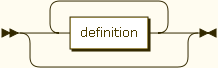
\includegraphics[scale=0.66]{grammar/grammar.png}

\item definition:

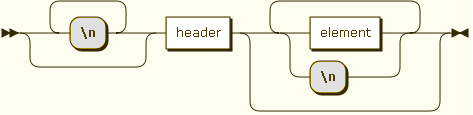
\includegraphics[scale=0.66]{grammar/definition.png}

\item header:

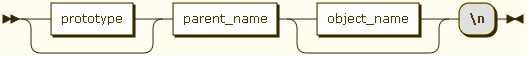
\includegraphics[scale=0.66]{grammar/header.png}

\item parent\_name:

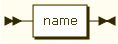
\includegraphics[scale=0.66]{grammar/name_xx.png}

\item object\_name:

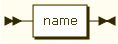
\includegraphics[scale=0.66]{grammar/name_xx.png}

\item element:

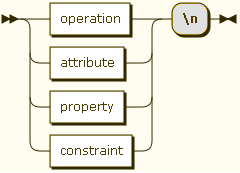
\includegraphics[scale=0.66]{grammar/element.png}
\end{itemize}
\subsection{Atrybuty}
\begin{itemize}
\item attribute:

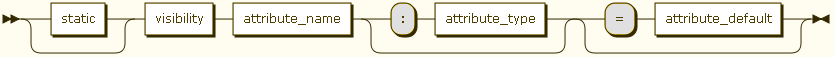
\includegraphics[scale=0.66]{grammar/attribute.png}

\item attribute\_name:

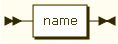
\includegraphics[scale=0.66]{grammar/name_xx.png}

\item attribute\_type:

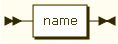
\includegraphics[scale=0.66]{grammar/name_xx.png}

\item attribute\_value:

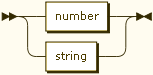
\includegraphics[scale=0.66]{grammar/attribute_value.png}
\end{itemize}
\subsection{Operacje}
\begin{itemize}
\item operation:

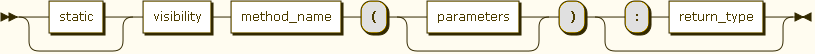
\includegraphics[scale=0.66]{grammar/operation.png}

\item operation\_name:

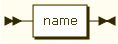
\includegraphics[scale=0.66]{grammar/name_xx.png}

\item return\_type:

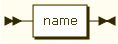
\includegraphics[scale=0.66]{grammar/name_xx.png}

\item parameters:

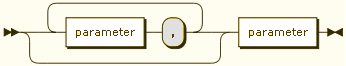
\includegraphics[scale=0.66]{grammar/parameters.png}

\item parameter:

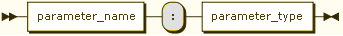
\includegraphics[scale=0.66]{grammar/parameter.png}

\item parameter\_name:

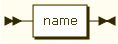
\includegraphics[scale=0.66]{grammar/name_xx.png}

\item parameter\_type:

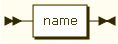
\includegraphics[scale=0.66]{grammar/name_xx.png}
\end{itemize}
\subsection{Właściwości}
\begin{itemize}
\item property:

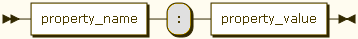
\includegraphics[scale=0.66]{grammar/property.png}

\item property\_name:

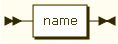
\includegraphics[scale=0.66]{grammar/name_xx.png}

\item property\_value:

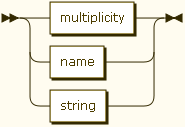
\includegraphics[scale=0.66]{grammar/property_value.png}
\end{itemize}
\subsection{Ograniczenia}
\begin{itemize}
\item constraint:

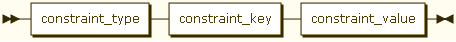
\includegraphics[scale=0.66]{grammar/constraint.png}

\item constraint\_type:

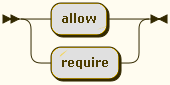
\includegraphics[scale=0.66]{grammar/constraint_type.png}

\item constraint\_key:

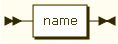
\includegraphics[scale=0.66]{grammar/name_xx.png}

\item constraint\_value:

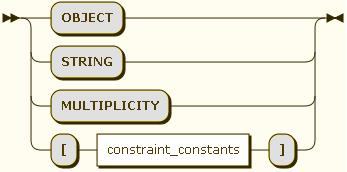
\includegraphics[scale=0.66]{grammar/constraint_value.png}

\item constraints\_constants:

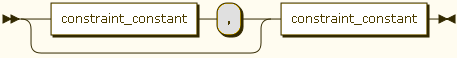
\includegraphics[scale=0.66]{grammar/constraint_constants.png}

\item constraint\_constant:

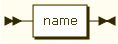
\includegraphics[scale=0.66]{grammar/name_xx.png}
\end{itemize}
\subsection{Generyczne}
\begin{itemize}
\item multiplicity:

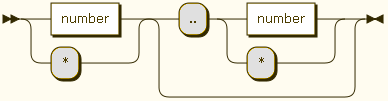
\includegraphics[scale=0.66]{grammar/multiplicity.png}

\item visibility:

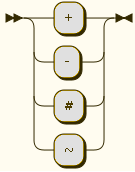
\includegraphics[scale=0.66]{grammar/visibility.png}

\item static:

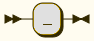
\includegraphics[scale=0.66]{grammar/static.png}

\item prototype:

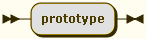
\includegraphics[scale=0.66]{grammar/prototype.png}

\item error:

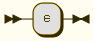
\includegraphics[scale=0.66]{grammar/error.png}
\end{itemize}
\subsection{pyparsing}
\begin{itemize}
\item number:

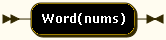
\includegraphics[scale=0.66]{grammar/number.png}

\item name:


\includegraphics[scale=0.66]{grammar/name.png}

\item string:

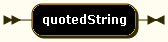
\includegraphics[scale=0.66]{grammar/string.png}
\end{itemize}